\subsection{Lab3: Audio}
%*********************
\begin{frame}{}

\pgfdeclareimage[width=\paperwidth,height=\paperheight]{bg}{imagenes/fondo_lab}
\setbeamertemplate{background}{\pgfuseimage{bg}}

\bfseries{\textrm{\LARGE Lab3\\ \Large Audio}}
\raggedright
\end{frame}
%*********************

\begin{frame}{Audio \index{Audio}}

\pgfdeclareimage[width=\paperwidth,height=\paperheight]{bg}{imagenes/fondo3}
\setbeamertemplate{background}{\pgfuseimage{bg}}


En esta práctica se generará un tono desde la tarjeta de sonido de la computadora, originado desde el software y emitido a través de los parlantes del computador, dicha señal será visualizada desde un osciloscopio, un FFT, y diagrama de cascada (espectrograma), realizando pruebas de "loopback" usando el micrófono de la computadora.

\end{frame}
%----------------

\begin{frame}{Diagrama:  “emisión de audio desde la computadora”\index{Audio}}

\begin{figure}

\begin{center}
\vspace{-0.3cm}
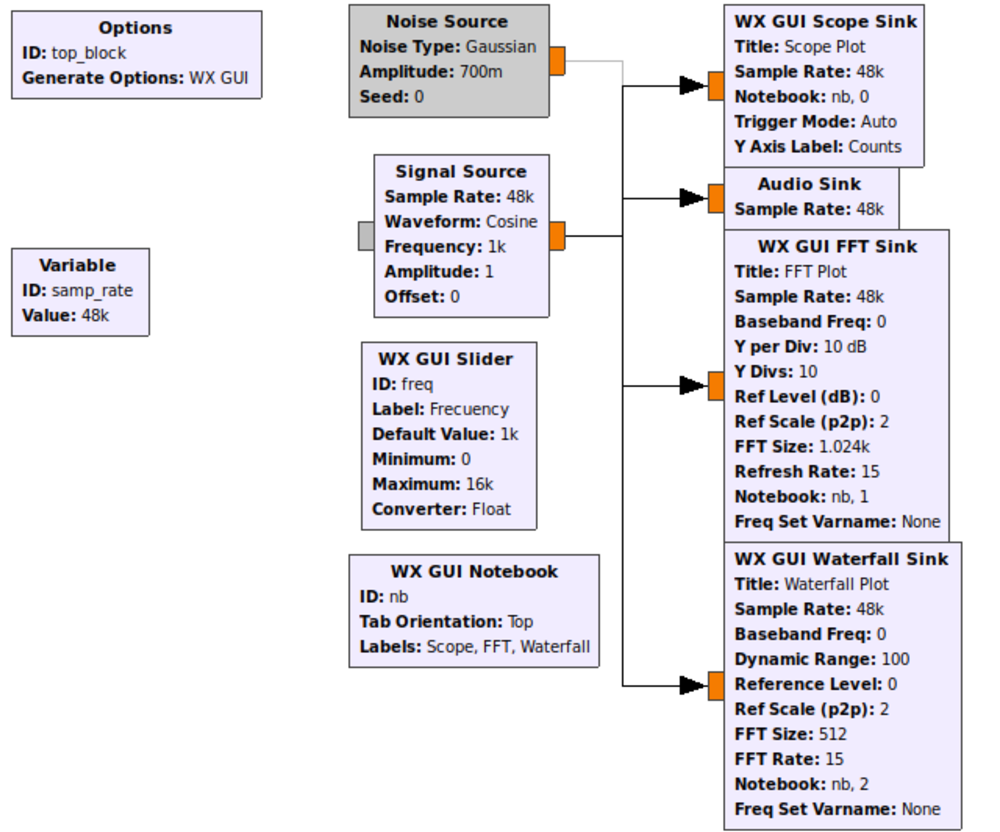
\includegraphics[width=.7\textwidth]{parte1/lab3/pdf/lab3_1.pdf}
\end{center}
\end{figure}

\end{frame}
%----------------

\begin{frame}{Diagrama:  “emisión de audio desde la computadora”\index{Audio}}

\begin{figure}

\begin{center}
\vspace{-2mm}
    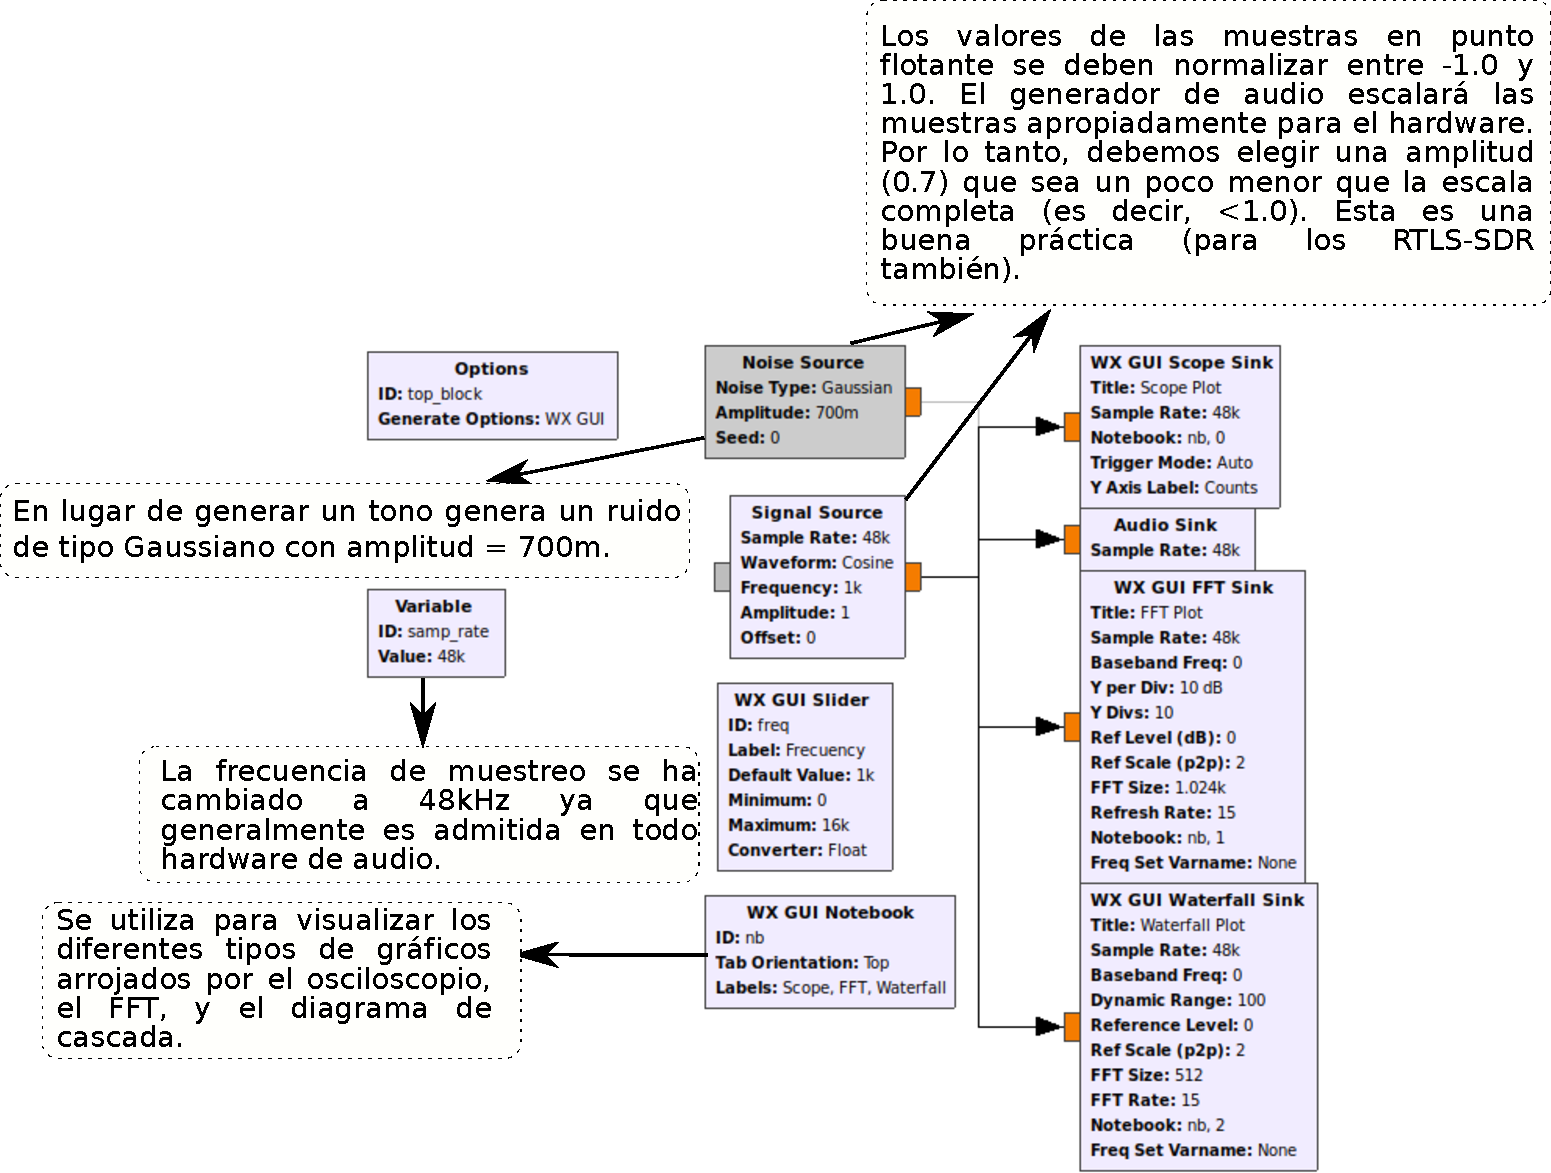
\includegraphics[width=.85\textwidth]{parte1/lab3/pdf/lab3_2.pdf}
\end{center}
\end{figure}

\end{frame}
%----------------

\begin{frame}{Diagrama:  “emisión de audio desde la computadora”\index{Audio}}

\begin{figure}

\begin{center}
\vspace{-1mm}
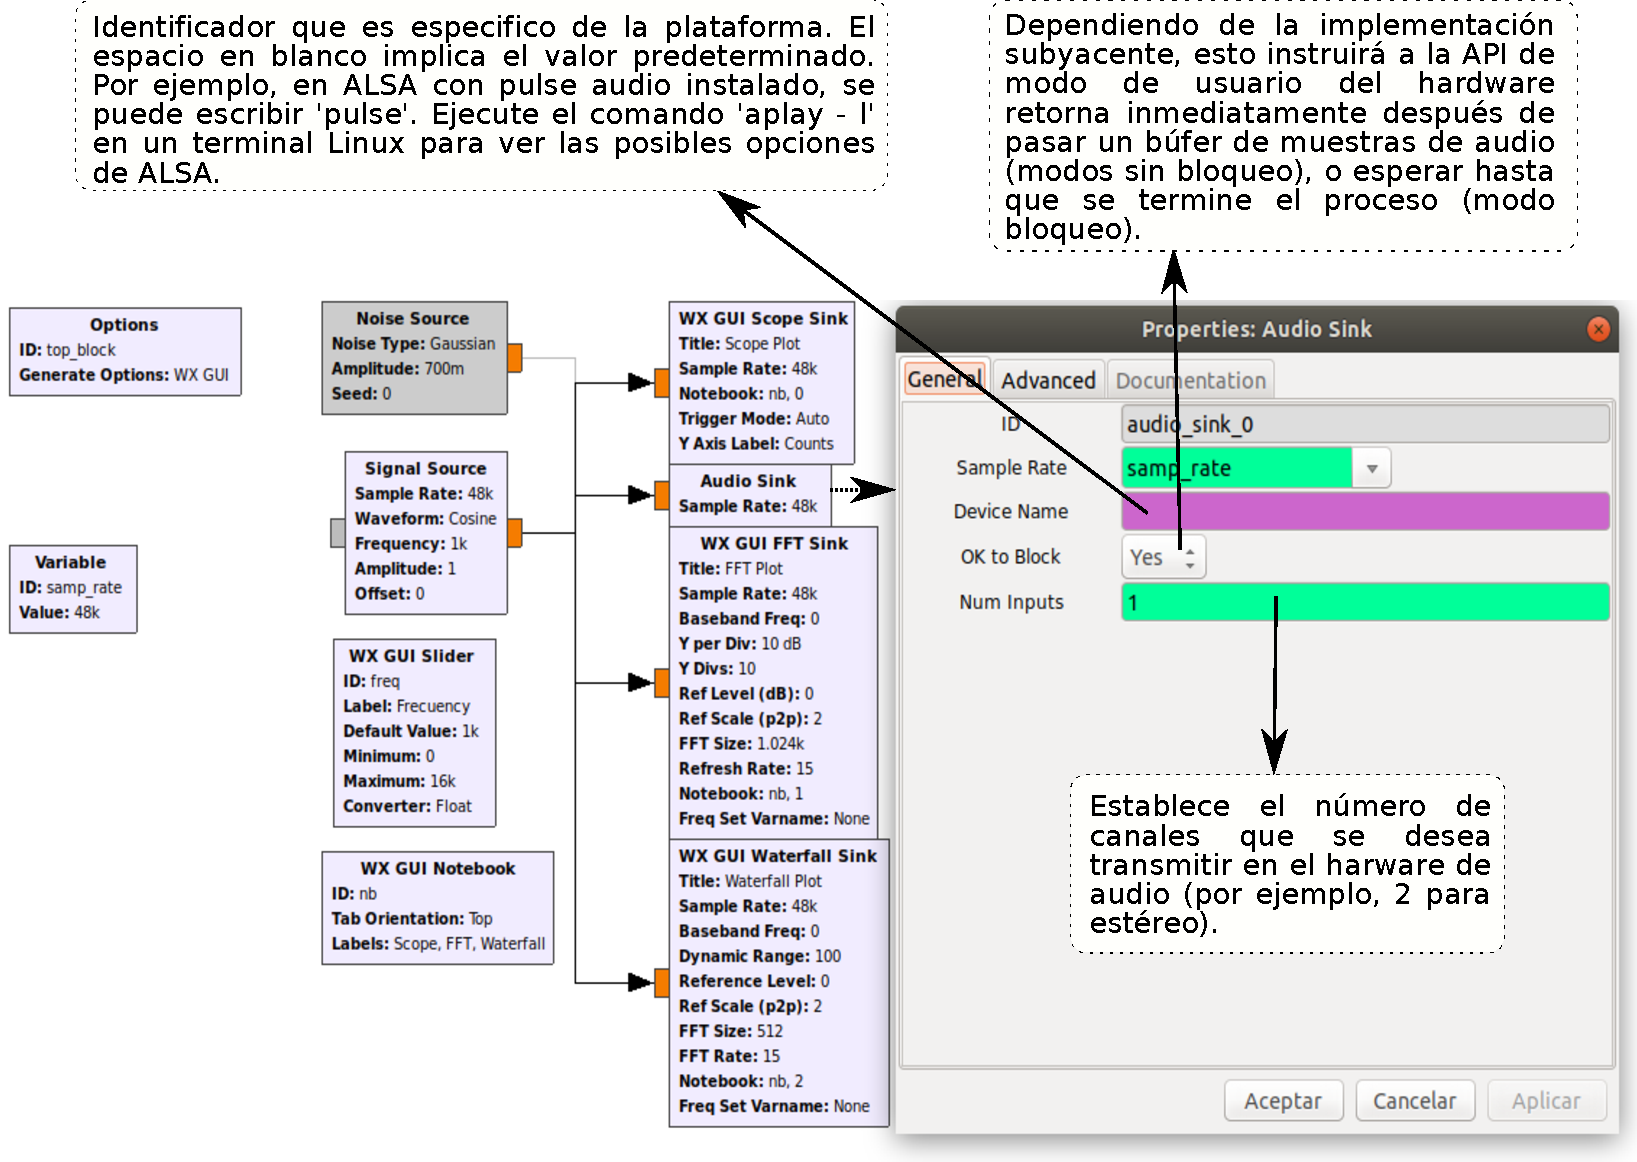
\includegraphics[width=.92\textwidth]{parte1/lab3/pdf/lab3_3.pdf}
\end{center}
\end{figure}

\end{frame}
%----------------

\begin{frame}{Diagrama:  “emisión de audio desde la computadora”\index{Audio}}

\begin{figure}

\begin{center}
\vspace{-8mm}
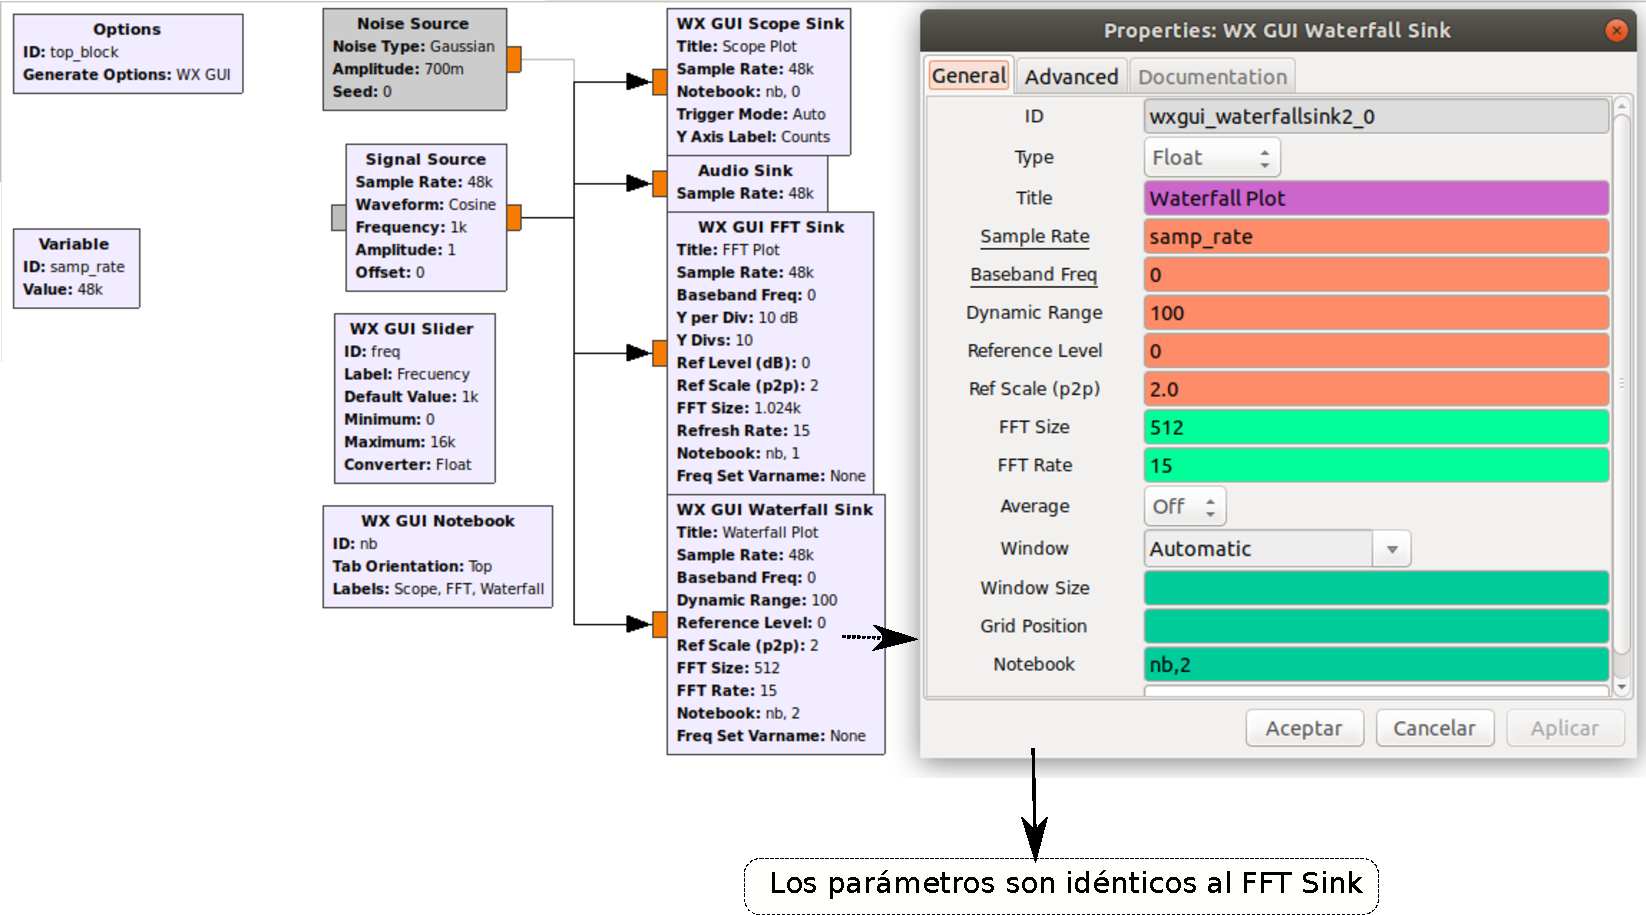
\includegraphics[width=1.05\textwidth]{parte1/lab3/pdf/lab3_4.pdf}
\end{center}
\end{figure}

\end{frame}
%----------------

\begin{frame}{Audio\index{Audio}}

Es importante saber que:\\
\begin{itemize}
    \item
    {Cuando Audio Sink es el único dispositivo hardware en el diagrama de bloques capaz de generar audio, el modo de bloqueo (‘OK to Block’) aplicará un regulador a la producción de muestras del sample\_rate, para que opere eficazmente al reproducir el sonido\cite{Seeber2014}.}
    \item
    {Esto puede ser problemático si la fuente del diagrama de flujo es, por ejemplo, un RTL-SDR. La fuente es también un hardware que tiene su propio reloj interno y será regulado a la tasa de producción de las muestras, mientras que el Audio Sink regula el uso con su propio reloj no sincronizado. Esto se llama el problema de “dos relojes".}
\end{itemize}
\end{frame}
%----------------

\begin{frame}{Audio\index{Audio}}
\begin{itemize}
    \item 
    {Para solucionar este problema de dos relojes, se coloca un regulador de audio en modo sin bloqueo (no dar click ‘Botón de Bloqueo’) de tal forma que nunca interrumpa el diagrama de bloque (es decir, no aplicar el regulador controlado). Esto usará muestras de forma normal, pero si hay un exceso (por ejemplo, el RTL-SDR está produciendo muestras un poco más rápido de lo que el Audio Sink puede usar), se perderán las muestras (podría causar fallas de audio).}
    \item 
    {Esto no soluciona el caso en el que las muestras se producen más lentamente que la tasa de uso del Audio Sink (esto producirá una ejecución lenta: el audio sonará agitado y se imprimirá ‘aU’ en la ventana de registro).}
\end{itemize}



\end{frame}
%----------------

\begin{frame}{Audio\index{Audio}}

\begin{figure}

\begin{center}
\vspace{-7mm}
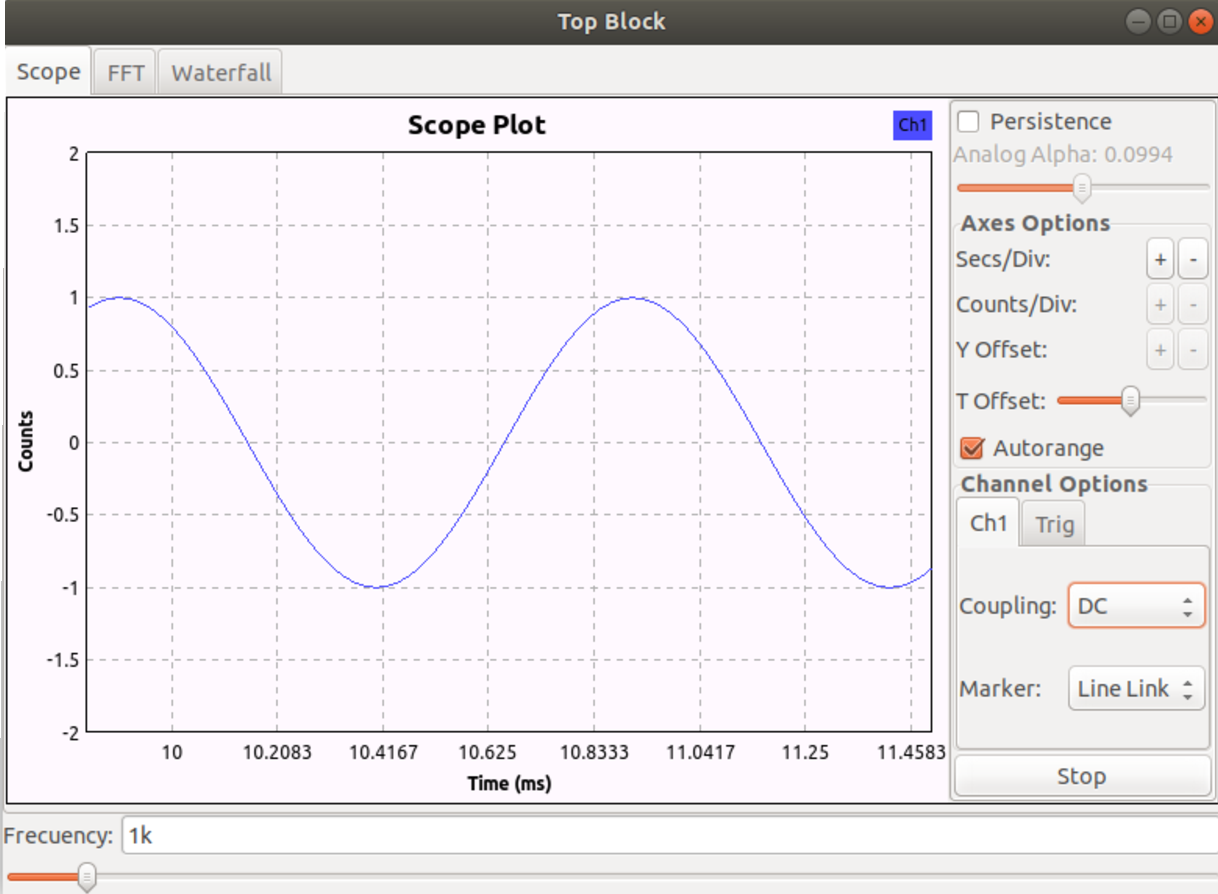
\includegraphics[width=\textwidth, height=0.6\paperheight]{parte1/lab3/pdf/lab3_5.pdf}
\end{center}
\end{figure}
%\tiny
\vspace{-4mm}
La misma onda seno de las prácticas anteriores, pero ahora se puede escuchar emitida por los parlantes del computador.
\end{frame}
%----------------

\begin{frame}{Audio\index{Audio}}

\begin{figure}

\begin{center}
\vspace{-6mm}
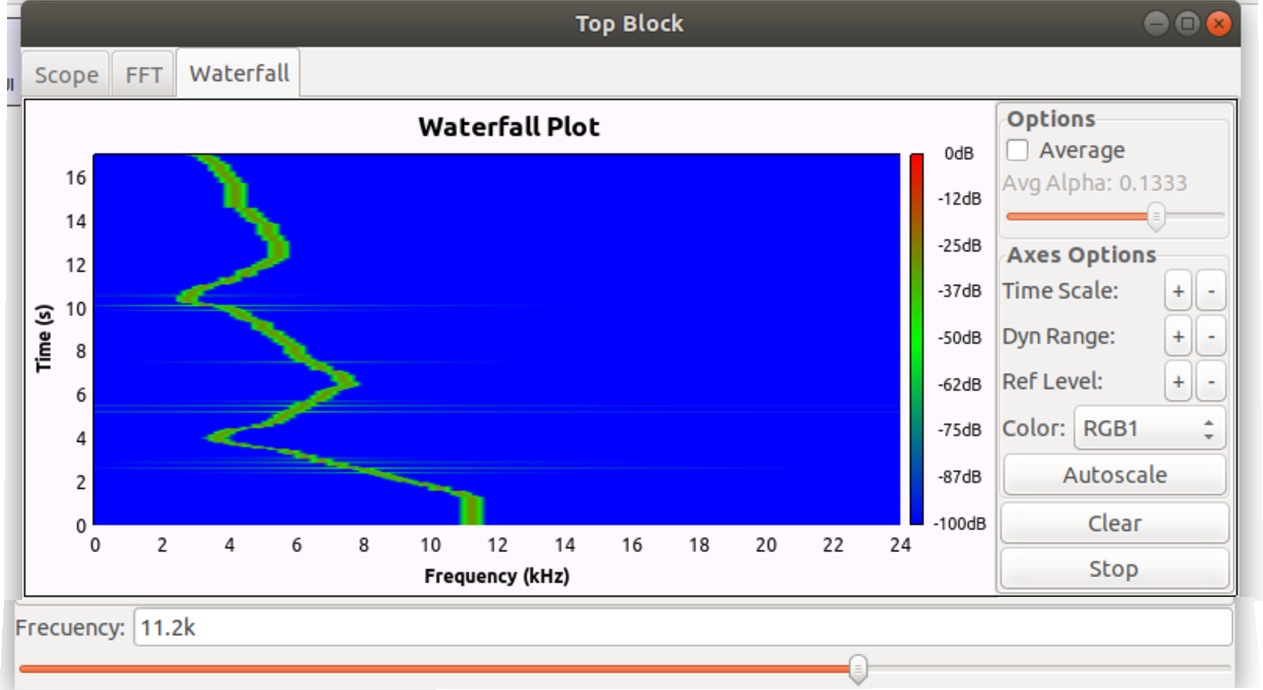
\includegraphics[width=0.8\textwidth]{parte1/lab3/pdf/lab3_6.pdf}
\end{center}
\end{figure}
\vspace{-3mm}

Visualiza el FFT que se desplaza en el tiempo mediante el diagrama de cascada (espectrograma) de la señal emitida. Se añade un bloque de prueba por medio de un generador de señales y un variador deslizante con lo cual se escucha el tono variado en el Audio Sink y poder ver la variación de la frecuencia en el diagrama de cascada.
\end{frame}
%----------------

\begin{frame}{Diagrama: recepción de audio\index{Audio}}

\begin{figure}

\begin{center}
%\vspace{-5mm}
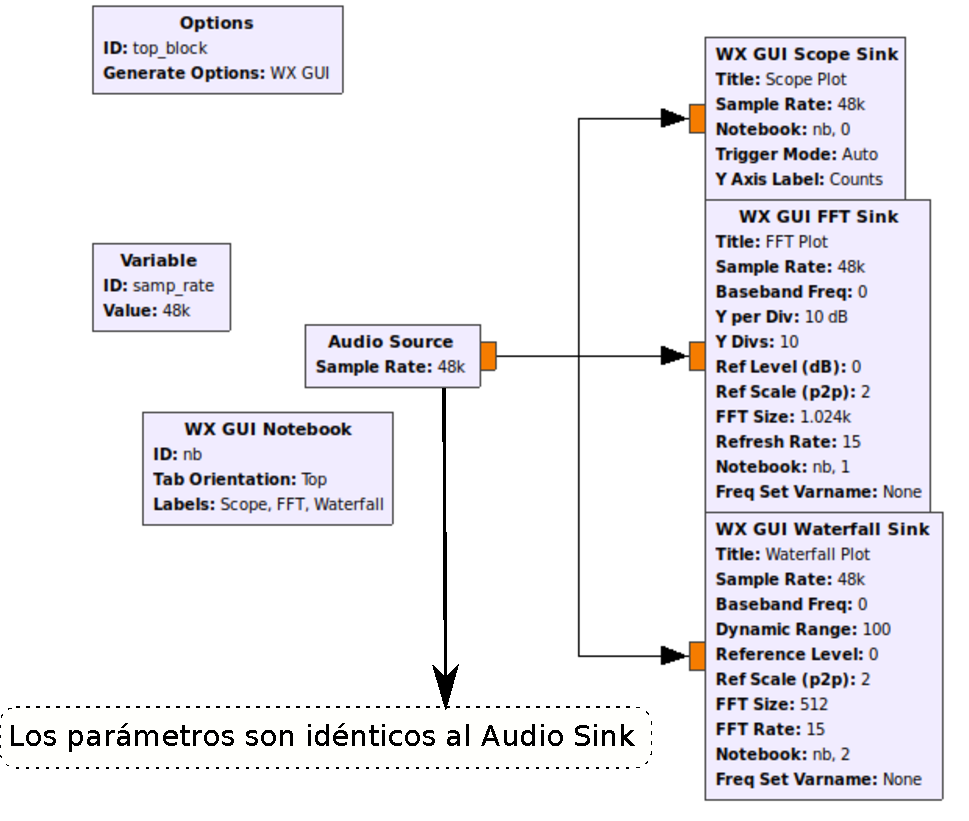
\includegraphics[width=.73\textwidth]{parte1/lab3/pdf/lab3_7.pdf}
\end{center}
\end{figure}

\end{frame}
%----------------

\begin{frame}{Audio\index{Audio}}

\begin{figure}
\begin{center}
\vspace{-8mm}
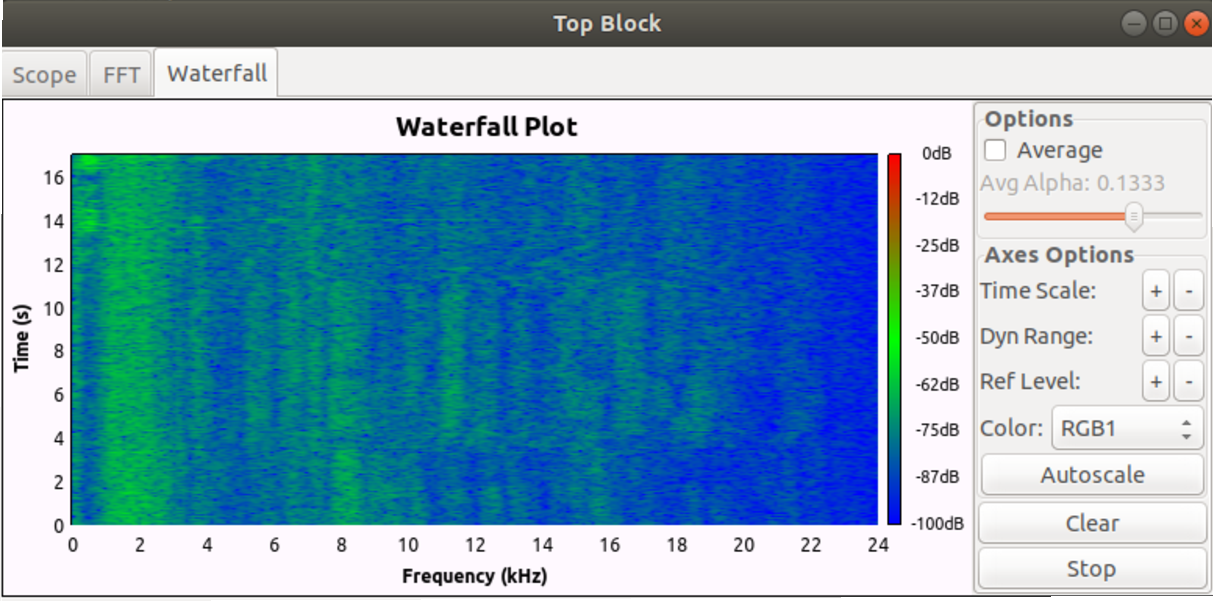
\includegraphics[width=\textwidth]{parte1/lab3/pdf/lab3_8.pdf}
\end{center}
\end{figure}

Muestra las diferentes señales presentes en el entorno captadas por la tarjeta de audio de la computadora a través del micrófono.

\end{frame}
%----------------

\begin{frame}{Diagrama: prueba con aproximación de “loopback”\index{Audio}}

\begin{figure}
\begin{center}
\vspace{-6mm}
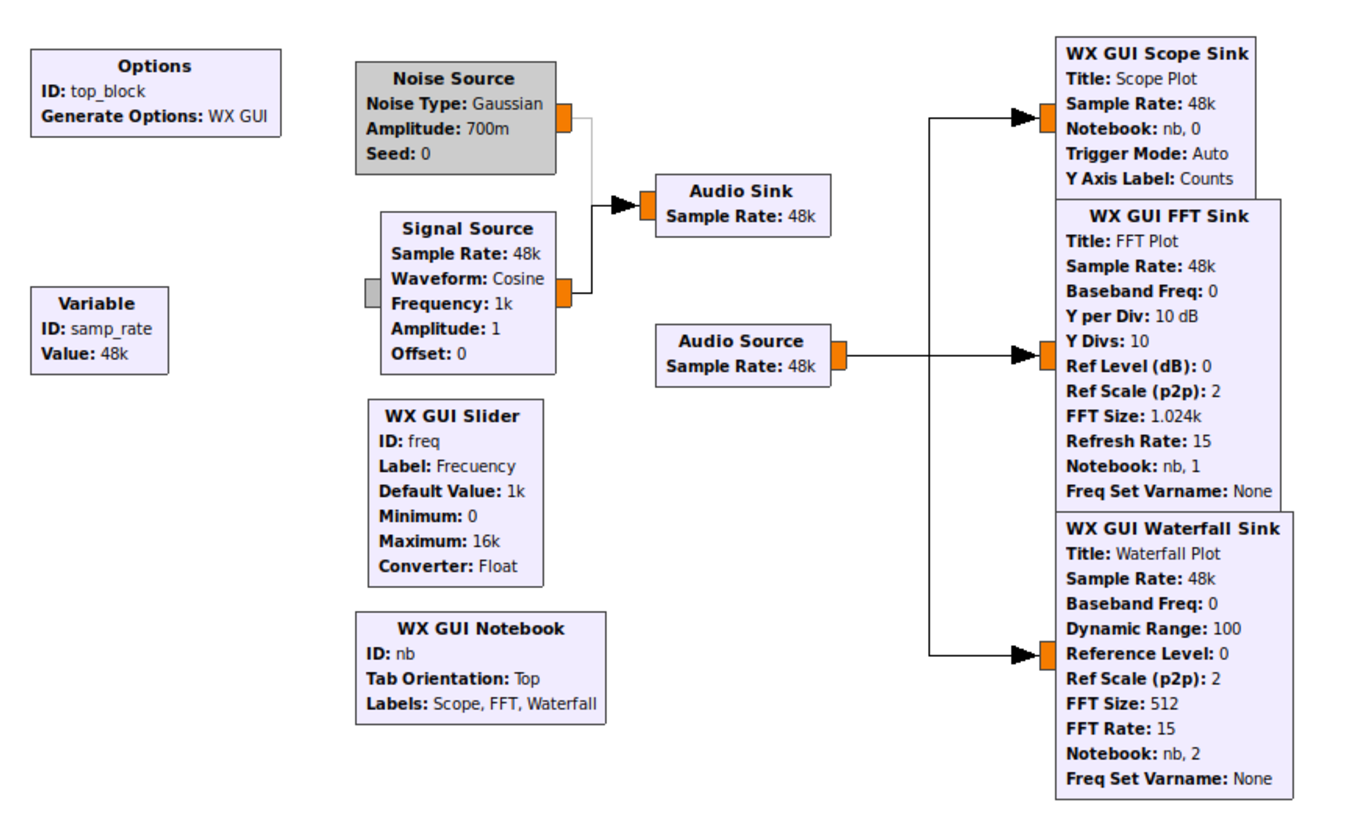
\includegraphics[width=\textwidth, height=0.6\paperheight]{parte1/lab3/pdf/lab3_9.pdf}
\end{center}
\end{figure}
\vspace{-5mm}
Ejecutando el programa generador de onda sinusoidal al mismo tiempo, y cambiando la frecuencia. Se trata de una prueba aproximada de “loopback" en la que el micrófono de la computadora escucha sus altavoces.

\end{frame}
%----------------

\begin{frame}{Audio\index{Audio}}

\begin{figure}
\begin{center}
\vspace{-8mm}
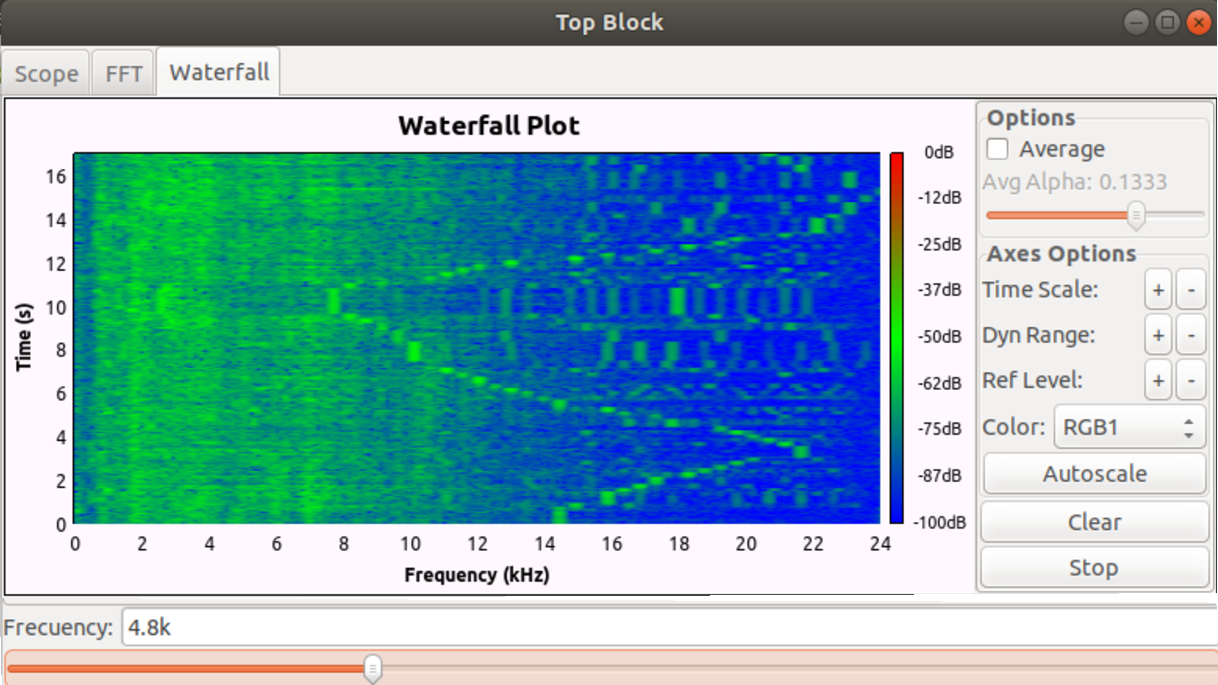
\includegraphics[width=\textwidth, height=0.6\paperheight]{parte1/lab3/pdf/lab3_10.pdf}
\end{center}
\end{figure}
\vspace{-5mm}
Con la realimentación de las entradas micrófono-altavoces y generación de señal a través de la tarjeta de audio de la computadora.

\end{frame}
%---------------
